% =====================================================================
% Person 2 -- text for Sections 3, 5.2, 6.2 and 7.2 + bibliography entries
% (same block format as person3_sections.tex)
% Figures (in report/): fig_5_2_network.png, fig_5_2_bridges.png
% Every number comes from notebooks/NA_02_RQ2.ipynb -> results/rq2_summary.json
% =====================================================================


% ---------------------------------------------------------------------
% BLOCK 1 -> Section 3 (replace the template text under \section{Datasets})
% ---------------------------------------------------------------------
%<<SECTION3
We use the public \emph{email-Eu-core} dataset from the Stanford Large
Network Dataset Collection (SNAP), built from the e-mails of a large European
research institution and first used to study network growth
\cite{leskovec2007} and community detection \cite{yin2017}. We did not
gather or digitise data: we downloaded the sender--receiver pairs and the
department of each member. The data is
anonymised and only covers e-mails between members. SNAP also offers a
timestamped version covering 803 days \cite{paranjape2017}; we use the static
one, since our questions concern who e-mails whom, not when.

\textbf{Networks.} We study five monomodal networks
(Table~\ref{tab:datasets}). Nodes are members of the institution, with one
attribute, their department (one of 42). A directed edge $u \rightarrow v$
exists if $u$ sent at least one e-mail to $v$; edges are unweighted. The
\emph{whole network} contains all 1{,}005 members. Each of the four
\emph{department networks} contains the members of one of the four largest
departments (4, 14, 1, 21) and only the e-mails among them (the induced
subgraph). SNAP's own timestamped department networks use different node IDs
and carry no department label, so we could not link them to our departments;
by building our own, node IDs are the same in all five networks. As a check,
SNAP's ``Dept3'' file has the same in- and out-degree sequences as our
department~14 without its three isolated members.

\textbf{Construction rules.} All group members built the networks with one
shared script: (i)~the 642 self-loops are removed, leaving 24{,}929 of the
25{,}571 listed edges; (ii)~isolated nodes are kept, since members who send
no e-mail still belong to the institution; (iii)~when a measure needs an
undirected network, two members are linked if at least one e-mailed the other
(OR rule); (iv)~every random procedure uses the seed 42.

\textbf{Tools.} We handled the data with Python (pandas, NumPy), computed all
measures with NetworkX 3.7 and drew figures with matplotlib, using the Gephi
layout algorithm ForceAtlas2 \cite{jacomy2014}. The notebooks are public at
\texttt{github.com/foadas/network-analysis-email-eu} and download the data
from SNAP, so every number can be reproduced.

\begin{table}[ht]
\centering
\small
\begin{tabular}{lrrrrr}
\toprule
 & Whole & Dept 4 & Dept 14 & Dept 1 & Dept 21 \\
\midrule
Nodes                        & 1005  & 109  & 92   & 65   & 61   \\
Edges (directed)             & 24929 & 1167 & 1506 & 502  & 601  \\
Edges (undirected, OR rule)  & 16064 & 745  & 973  & 331  & 355  \\
Isolated nodes               & 19    & 8    & 3    & 6    & 15   \\
\bottomrule
\end{tabular}
\caption{The five networks. A member isolated in a department network may
still e-mail other departments.}
\label{tab:datasets}
\end{table}
%>>SECTION3


% ---------------------------------------------------------------------
% BLOCK 2 -> Section 5.2 (replace "% TODO (Person 2)" under \subsection{Central actors and bridges (RQ2)})
% ---------------------------------------------------------------------
%<<SECTION52
We computed six centrality measures on the directed whole network and the
k-core on its undirected version \cite{newman2018,borgatti2018}.
\emph{In-degree} counts the colleagues a member receives e-mail from;
\emph{out-degree} those they write to, marking broadcasters.
\emph{PageRank} \cite{brin1998} ($\alpha=0.85$) weights e-mails received
from members who are themselves often written to (prestige). In \emph{HITS}
\cite{kleinberg1999}, a high \emph{authority} score means that many active
senders write to a member, and a high \emph{hub} score that they write to
many authorities. \emph{Betweenness} \cite{freeman1977} (exact, following
e-mail direction) is the share of shortest paths between other members that
pass through a member: brokers who can pass on or hold back information. The
\emph{core number} is the largest $k$ such that a member belongs to a group
where everyone has at least $k$ contacts; the highest value marks the
institution's dense centre. We dropped closeness centrality because only 80\%
of members can reach each other following e-mail direction, so many distances
are undefined.

\textbf{Who is central.} The same few people top every measure
(Table~\ref{tab:top10}): only 17 different members fill the 60 positions,
and member~160 is first on all six, with contacts in 35 other departments.
Department~36 stands out: with 22 members (2.2\%) it holds 32 of the 60
positions and 19.5\% of all betweenness. Its members are both authorities and
hubs, consistent with the service role suggested in
Section~\ref{sec:departments}. Most other names come from departments 4, 25
and 34. Brokerage is very unequal: the Gini coefficient of betweenness is
0.81, and the top ten members (1\% of the institution) hold 21\% of it. The
innermost core ($k=34$) has 79 members from 28 departments, including 14 of
the 22 members of department~36.

The rankings agree closely (Table~\ref{tab:spearman}): Spearman correlations
among the seven centrality measures range from 0.83 to 0.98. Here the measures
describe one dimension, overall activity, rather than distinct roles.

\textbf{Who bridges departments.} Betweenness does not show \emph{which}
boundaries a member crosses, so we combined it with the \emph{external
share}, the share of a member's contacts in other departments. It is only
weakly related to centrality (last row of Table~\ref{tab:spearman}). We call
a member a \emph{bridge} if their betweenness is in the top 10\% and their
external share in the top 25\% (at least 0.80), and an \emph{internal broker}
if only betweenness is high. To test whether brokers reach outside their
department more than others (H0: no association between betweenness and
external share), we shuffled external shares among the 986 members with at
least one contact 5{,}000 times. The top 10\% by betweenness have 77\% of
their contacts outside their department, against 51\% for the others
(Spearman $\rho=0.24$), a significant difference ($p=0.0002$).

Of these 101 members, 50 are bridges from 19 departments
(Figure~\ref{fig:bridges}). The strongest are the members of department~36
and members 5 and 64 (department~25) and 434 (department~34), each with over
90\% of their contacts outside their department, reaching 30 or more of the
41 other departments. The other 51 are internal brokers, most clearly in
department~14, the most closed department (Section~\ref{sec:departments}):
members 44 and 498 have high betweenness but only 49\% and 41\% of their
contacts outside it, so they hold their department together rather than
connect it. Members 129 and 183 play this role in department~4.
Figure~\ref{fig:network} places both groups in the network.

Finally, does contact between departments depend on the bridges? Of the 861
department pairs, 641 are linked by at least one edge. Removing the ten
strongest bridges leaves 630 linked, against 638 on average when removing
ten random members (100 draws; 7\% lost as many), and the average shortest
path grows only from 2.59 to 2.69. Even without all of department~36, 601
pairs stay linked. Bridges shorten paths, but department pairs are linked
through many members.

\begin{table}[ht]
\centering
\small
\begin{tabular}{rllllll}
\toprule
Rank & In-degree & Out-degree & PageRank & Hub & Authority & Betweenness \\
\midrule
1 & \textbf{160 (36)} & \textbf{160 (36)} & \textbf{160 (36)} & \textbf{160 (36)} & \textbf{160 (36)} & \textbf{160 (36)} \\
2 & \textbf{62 (36)} & \textbf{82 (36)} & \textbf{62 (36)} & \textbf{82 (36)} & \textbf{107 (36)} & \textbf{86 (36)} \\
3 & \textbf{107 (36)} & \textbf{121 (36)} & \textbf{86 (36)} & \textbf{121 (36)} & \textbf{62 (36)} & 5 (25) \\
4 & \textbf{121 (36)} & \textbf{107 (36)} & \textbf{107 (36)} & \textbf{107 (36)} & 434 (34) & \textbf{121 (36)} \\
5 & \textbf{86 (36)} & \textbf{86 (36)} & \textbf{121 (36)} & \textbf{62 (36)} & \textbf{121 (36)} & \textbf{62 (36)} \\
6 & 434 (34) & \textbf{62 (36)} & 5 (25) & 249 (14) & 183 (4) & \textbf{107 (36)} \\
7 & 183 (4) & 13 (26) & 129 (4) & 434 (34) & 128 (5) & 64 (25) \\
8 & 129 (4) & 249 (14) & 183 (4) & 183 (4) & 256 (4) & \textbf{82 (36)} \\
9 & 64 (25) & 183 (4) & 64 (25) & \textbf{86 (36)} & 249 (14) & 377 (7) \\
10 & 128 (5) & 434 (34) & 434 (34) & 114 (10) & 129 (4) & 129 (4) \\
\bottomrule
\end{tabular}
\caption{Ten most central members per measure, as \emph{member
(department)}; department~36 in bold.}
\label{tab:top10}
\end{table}

\begin{table}[ht]
\centering
\small
\begin{tabular}{lrrrrrrr}
\toprule
 & In & Out & PR & Hub & Auth & Betw & Core \\
\midrule
Out & 0.90 &  &  &  &  &  &  \\
PR & 0.98 & 0.89 &  &  &  &  &  \\
Hub & 0.88 & 0.97 & 0.86 &  &  &  &  \\
Auth & 0.96 & 0.85 & 0.91 & 0.89 &  &  &  \\
Betw & 0.88 & 0.94 & 0.90 & 0.90 & 0.83 &  &  \\
Core & 0.97 & 0.92 & 0.94 & 0.92 & 0.95 & 0.87 &  \\
External share & 0.25 & 0.24 & 0.20 & 0.32 & 0.38 & 0.24 & 0.30 \\
\bottomrule
\end{tabular}
\caption{Spearman correlations between measures (986 members with at least
one contact; PR = PageRank, Auth = authority, Betw = betweenness, Core = core
number); all $p<0.001$.}
\label{tab:spearman}
\end{table}

\begin{figure}[ht]
\centering
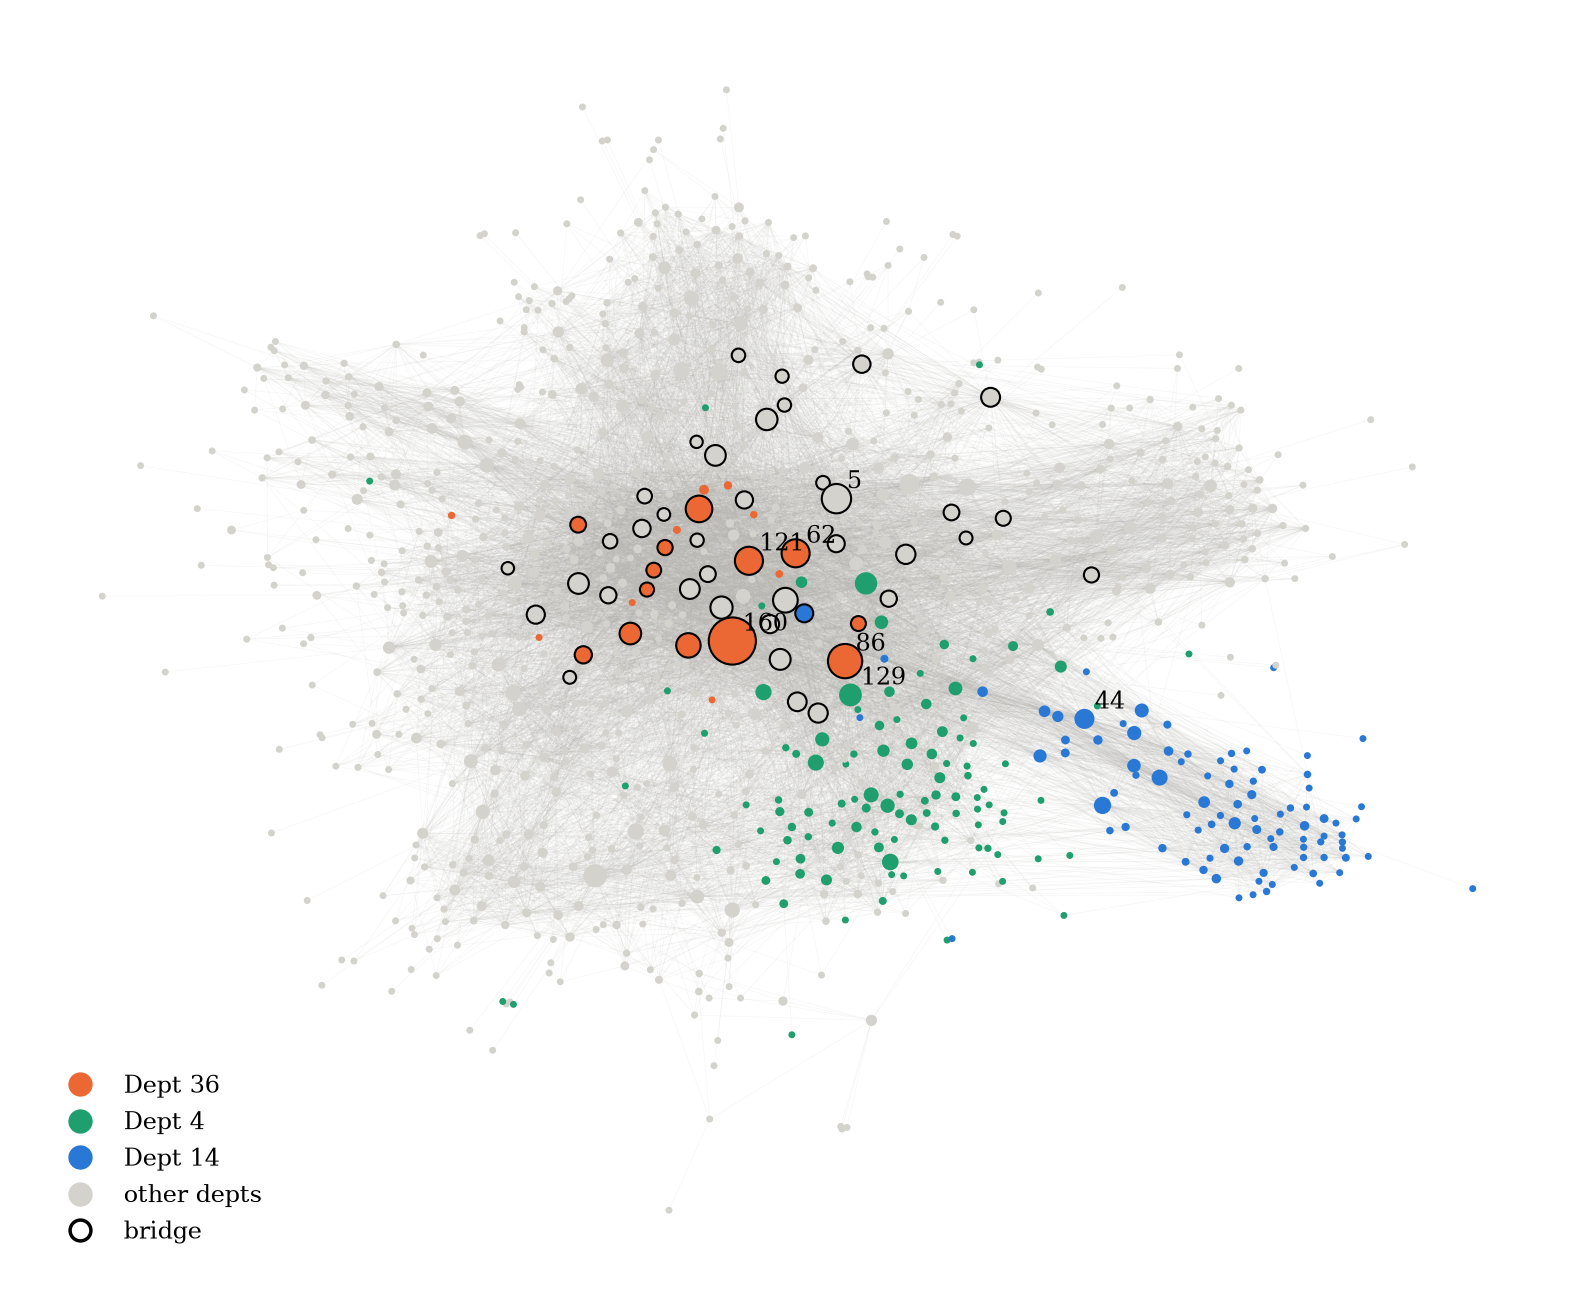
\includegraphics[width=0.8\textwidth]{fig_5_2_network.png}
\caption{Whole network (largest connected component, ForceAtlas2). Colour =
department, size = betweenness, black ring = bridge. Department~36 (orange)
sits at the centre, between all departments.}
\label{fig:network}
\end{figure}

\begin{figure}[ht]
\centering
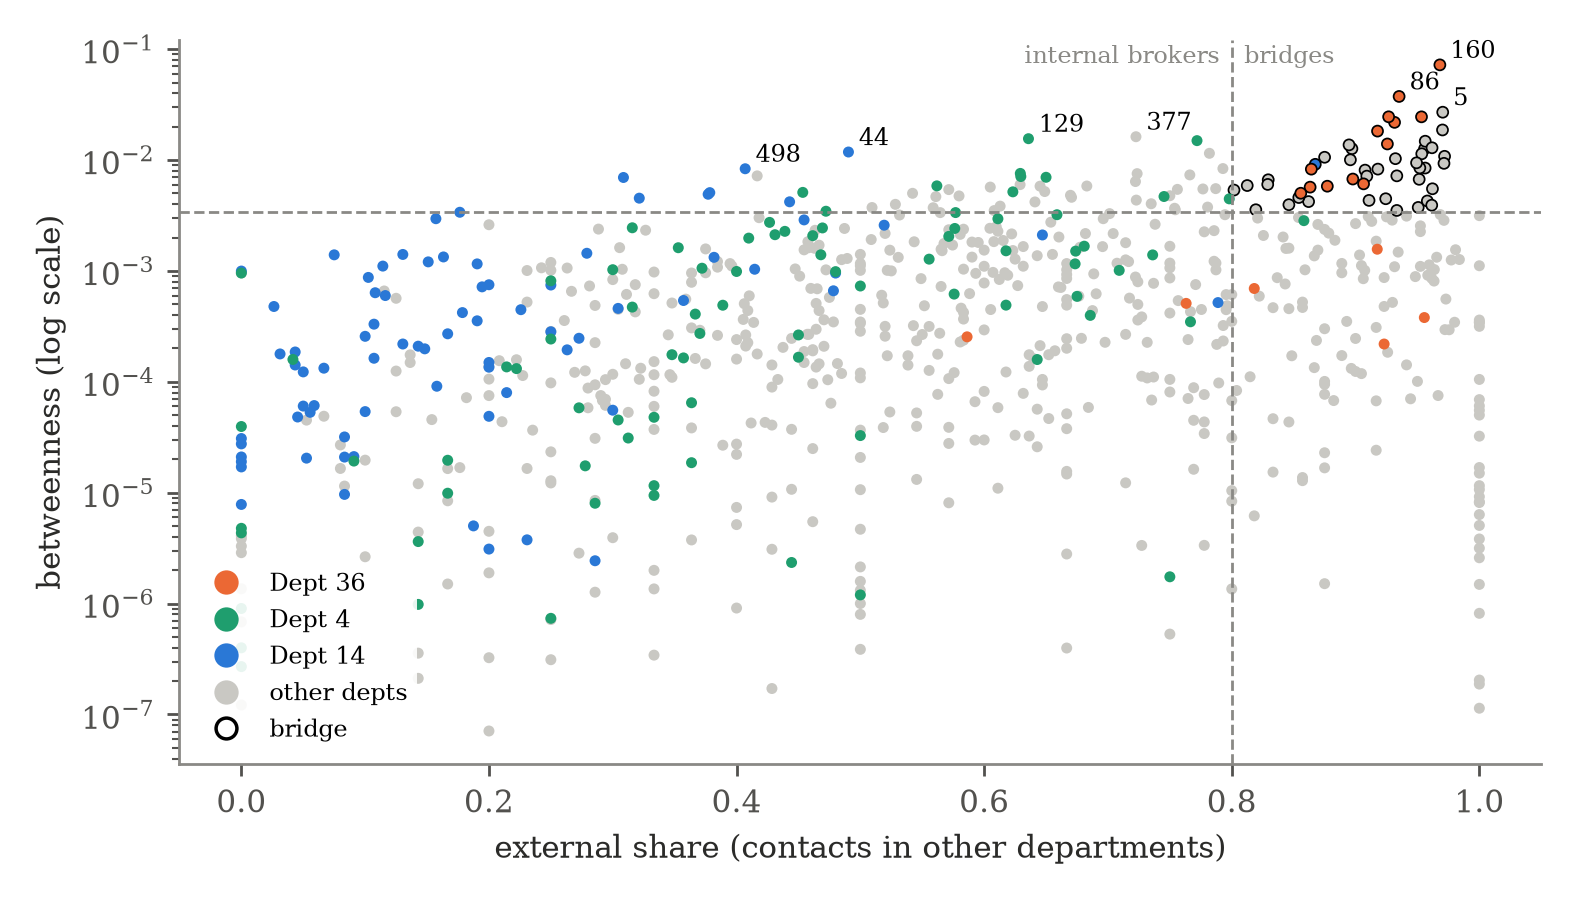
\includegraphics[width=0.85\textwidth]{fig_5_2_bridges.png}
\caption{External share against betweenness (log scale; 216 members with
betweenness 0 not shown). Dashed lines: thresholds. Top right: bridges; top
left: internal brokers, such as members 44 and 498 of department~14.}
\label{fig:bridges}
\end{figure}
%>>SECTION52


% ---------------------------------------------------------------------
% BLOCK 3 -> Section 6.2 (replace "% TODO 6.2 (Person 2), 6.3 (Person 3)": put this BEFORE Person 3's 6.3)
% ---------------------------------------------------------------------
%<<SECTION62
\subsection{RQ2: central actors and bridges}
A small, stable group holds the central positions: whoever writes to many
colleagues is also written to by many and lies on many paths. The clearest
centre is department~36, whose members fill half of all top-ten positions,
sit in the innermost core and write to almost every department, acting as a
service unit for the institution. Bridges between departments are mainly
these members and a few others from small departments, and members with high
betweenness reach clearly more outside their department than others. Large
or closed departments, such as 4 and 14, have instead internal brokers who
connect their own colleagues. Contact between departments does not depend on
the bridges, however: without them, almost all department pairs remain
linked.
%>>SECTION62


% ---------------------------------------------------------------------
% BLOCK 4 -> Section 7.2 (replace "% TODO 7.2 (Person 2), 7.3 (Person 3)": put this BEFORE Person 3's 7.3)
% ---------------------------------------------------------------------
%<<SECTION72
\subsection{RQ2: central actors and bridges}
First, edges are unweighted: one e-mail counts as much as daily contact, so
degree shows how many people a member reaches, not how much they write;
weights from the timestamped data could change the rankings. Second,
betweenness counts only shortest paths and ignores timing, while information
also travels along longer paths. Third, the bridge thresholds (top 10\% and
25\%) are our choice and would change who is called a bridge, although the
permutation test does not depend on them. Finally, we cannot verify that
department~36 really has a service role, since departments are the only
attribute available.
%>>SECTION72


% ---------------------------------------------------------------------
% BLOCK 5 -> bibliography (add before \end{thebibliography})
% (borgatti2018, newman2018, leskovec2007, yin2017 are already in main.tex)
% ---------------------------------------------------------------------
%<<BIB
\bibitem{brin1998} S.~Brin, L.~Page. The anatomy of a large-scale
  hypertextual web search engine. \emph{Computer Networks and ISDN Systems},
  30(1--7):107--117, 1998.
\bibitem{freeman1977} L.~C. Freeman. A set of measures of centrality based on
  betweenness. \emph{Sociometry}, 40(1):35--41, 1977.
\bibitem{jacomy2014} M.~Jacomy, T.~Venturini, S.~Heymann, M.~Bastian.
  ForceAtlas2, a continuous graph layout algorithm for handy network
  visualization designed for the Gephi software. \emph{PLoS ONE},
  9(6):e98679, 2014.
\bibitem{kleinberg1999} J.~M. Kleinberg. Authoritative sources in a
  hyperlinked environment. \emph{Journal of the ACM}, 46(5):604--632, 1999.
\bibitem{paranjape2017} A.~Paranjape, A.~R. Benson, J.~Leskovec. Motifs in
  temporal networks. In \emph{Proceedings of the Tenth ACM International
  Conference on Web Search and Data Mining}, 2017.
%>>BIB
